%\section[Gas \Cherenkov{} Counters]{Gas \Cherenkov{} Counters
\chapter[Gas \Cherenkov{} Counters]{Gas \Cherenkov{} Counters
\footnote{
  $CVS~revision~ $Id: gas-cer.tex,v 1.6 2005/04/04 22:27:25 gen Exp $ $
}
\footnote{Author: B. B. Wojtsekhowski \email{bogdanw@jlab.org}}
}

A gas \Cherenkov{} detector filled  with CO$_{2}$ at atmospheric 
pressure is mounted between the trigger scintillator planes S1 and S2. 
The detector has an electron identification efficiency 
of 99\% and a threshold for pions of 4.8 GeV/$c$.
The detector has ten spherical mirrors with 80 cm focal length, each
viewed by a PMT (ET Enterprises tube 9390KB); the light-weight mirrors
were developed at INFN.
The focusing of the \Cherenkov{} ring onto a
small area of the PMT photo-cathode leads to a high current-density  near
the anode. To prevent a non-linear PMT response, even in the case of few
photoelectrons, requires a progressive HV divider.
The length of the particle path in the gas radiator is 130 cm for the gas
\Cherenkov{} in the HRS-R, leading to an average of about twelve photoelectrons.
In the HRS-L, the gas \Cherenkov{} detector in its standard configuration has
a path length of 80~cm, yielding seven photoelectrons on average.
The total amount of material in the particle path is about 1.4\% $X_0$.

\section[Concept of the design]{Concept of the design}

Two similar threshold gas \Cherenkov{} counters have been constructed 
as a part of the particle identification equipment to be included 
in the focal plane detector package of the High Resolution Spectrometers (HRS) 
in the TJNAF experimental Hall A%
\infolevfour{ (see Fig.~\ref{fig:gas-counter})}. 
Each counter's housing is made of steel with thin entry and 
exit windows made of Tedlar\texttrademark{}.
Light-weight spherical mirrors have also been built, resulting in 
a very thin total thickness traversed by particles. 
%
\infolevfour{
\begin{figure}[p]
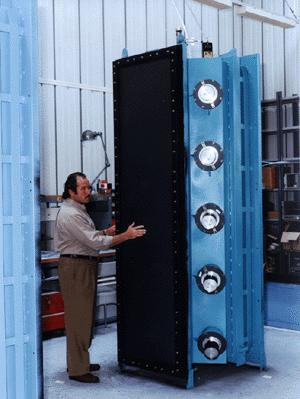
\includegraphics[angle=0,width=14cm]{gas_cer_fig1}
\caption[Gas \Cherenkov{} counter]
{Gas \Cherenkov{} counter.}
\label{fig:gas-counter}
\end{figure}
}

These two counters have identical sections but different lengths of 
the gas radiator, 80 cm for the left arm and 130 cm for the right arm. 
There is an additional section 50 cm long which can be attached to 
the short counter if needed.
Each \Cherenkov{} is made of 10  tubes (PMT) and 10 spherical mirrors. 
Each mirror has a rectangular shape, the radius of a curvature of the reflective
surface is 80~cm. %and  built in a empty sphere of interior radius 
%(reflective face) of 80 cm and thickness of 1 cm. 
%Each mirror has a rectangular profile built in a empty sphere of interior radius 
%(reflective face) of 80 cm and thickness of 1 cm. 
The mirror is 1~cm thick, it is built of a very light honeycomb structure, which
consists of the following materials:  
%The very light structure of the mirror is built like honeycomb 
%and is constituted as the following manner: 
the MgF$_2$ layer, which protects 
the aluminum; the aluminum, which assures the reflectivity; 
the plexiglas, which assures a good surface; and  
a sandwich backing (carbon-epoxy, phenolic honey comb, carbon epoxy), 
which assures the rigidity of the mirror. 

The 10 mirrors are placed just before the output window and are grouped in 
two columns of 5 mirrors. 
Each mirror reflects the light on a PMT placed at the side of the box. 
The mirrors of the same column are identical and the two columns are 
almost symmetrical. 
The positions and angles of the PMTs are not placed regularly, as like the mirrors, 
but were adjusted by an optical study in order to maximize the collection of light 
coming from the particular envelope of particles to be detected.
The PMTs are fixed and mirrors orientation can be adjusted by hand. 

The alignment procedure uses a small light source located about 820 cm
from the mirror plane on the symmetry axis of the counter.
\infolevfour{
The pictures in figs~\ref{fig:mirror-1} and~\ref{fig:mirror-6} 
show the image of the small light source on the PMT photo-cathodes during 
the mirror alignment procedure. 
%
\begin{figure}[p]
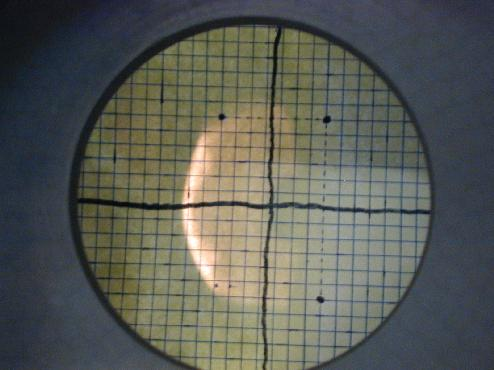
\includegraphics[angle=0,width=10cm]{gas_cer_fig3}
\caption[The image from mirror \#1 on PMT photo-cathode]
{ The image from the mirror \#1 on the PMT photo-cathode.}
\label{fig:mirror-1}
\end{figure}
%
\begin{figure}[p]
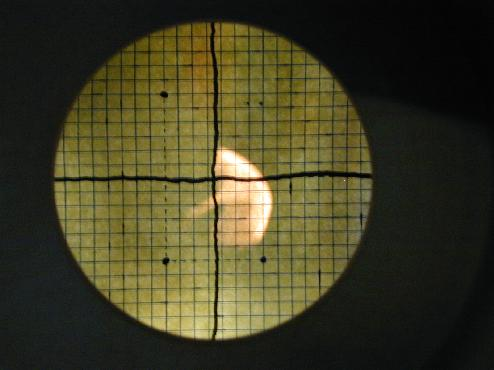
\includegraphics[angle=0,width=10cm]{gas_cer_fig2}
\caption[The image from mirror \#6 on PMT photo-cathode]
{ The image from the mirror \#6 on the PMT photo-cathode.}
\label{fig:mirror-6}
\end{figure}
}

The five photomultiplier tubes are fixed to the two side walls. 
Each one is surrounded by high magnetic-permeability shielding (mu-metal). 
The fixing provides high voltage insulation between the PMT and the steel vessel. 
A set of optical fibers provides light pulses to each PMT for their calibration. 

\section{Safety Assessment}

\begin{safetyen}{10}{10}
The PMTs are under high voltage and care is required when handling any 
components of the counter. The body of the \Cherenkov{} counter must be grounded. 
\end{safetyen}

\infolevtwo{
\section{Operating Procedure}

\paragraph{Operating Voltage}

%Modified by K. Allada %
%HV ratings for new ET Enterprise tubes %
\begin{safetyen}{10}{10}
The maximum operating voltage on the PMTs is about -2,000 V, but
nominally they are operated around -1,000 V. The voltage must be set to
zero before the HV cable will be connected or disconnected from HV divider.
The HV cables must be disconnected from all HV dividers before the replacement
of any PMT on the gas \Cherenkov{} counter. 
\end{safetyen}

The high voltage has to be adjusted in order to have 
the position of the photoelectron peak for each PMT at the same place, 
which is around 100 channels above the pedestal. 
For a good PMT the noise counting rate should not exceed 10 kHz.
Past experience shows that PMTs need to be replaced on average
every three years due to aging. Such a short life-time is about 3-4 
times less than normal, due to He content in Hall A,
which leads to a loss of the PMT's quantum efficiency.
} %infolev
 
\begin{safetyen}{10}{15}
\section{Responsible Personnel} 
\end{safetyen}

The individuals responsible for the operation 
of the gas \Cherenkov{} counters are given in Table \ref{tab:gas-cher:personnel}.

\begin{namestab}{tab:gas-cher:personnel}{Gas-\Cherenkov{}: authorized personnel}{%
      Gas-\Cherenkov{}: authorized personnel.}
  \BogdanWojtsekhowski{\em Contact}
  \JackSegal{}
\end{namestab}

% $Header: /group/halla/analysis/cvs/tex/osp/src/hrs_det/gas-cer.tex,v 1.6 2005/04/04 22:27:25 gen Exp $
% $Id: gas-cer.tex,v 1.6 2005/04/04 22:27:25 gen Exp $
% $Author: gen $
% $Date: 2005/04/04 22:27:25 $
% $Name:  $
% $Locker:  $
% $Log: gas-cer.tex,v $
% Revision 1.6  2005/04/04 22:27:25  gen
% Chnges after the review
%
% Revision 1.5  2003/12/17 03:59:48  gen
% authorized personnel tables unfied
%







